\documentclass[margin=0px]{article}

\usepackage{listings}
\usepackage[utf8]{inputenc}
\usepackage{graphicx}
\usepackage{float}
\usepackage[a4paper, margin=1in]{geometry}
\usepackage{amsthm}
\usepackage{amssymb}
\usepackage{t1enc}

\newenvironment{tetel}[1]{\paragraph{#1 \\}}{}
% A dokument itt kezdődik

\title{Záróvizsga tételsor \\ \large 13. Alapvető algoritmusok és adatszerkezetek}
\date{}
\author{Fekete Dóra}

\begin{document}

	\maketitle
	
	\begin{tetel}{Alapvető algoritmusok és adatszerkezetek}
			Egyszerű adattípusok ábrázolásai, műveletei és fontosabb alkalmazásai. A hatékony adattárolás és visszakeresés néhány megvalósítása (bináris keresőfa, AVL-fa, 2-3-fa és B-fa, hasítás (,,hash-elés”)). Összehasonlító rendező algoritmusok (buborék és beszúró rendezés, ill. verseny, kupac, gyors és összefésülő rendezés); a műveletigény alsó korlátja.
	\end{tetel}
	
	\section{Egyszerű adattípusok ábrázolásai, műveletei és fontosabb alkalmazásai}
	
	\subsection{Adattípus}
	
	\textit{Adatszerkezet}: $\sim$ struktúra. \\
	\textit{Adattípus}: adatszerkezet és a hozzá tartozó műveletek. \\
	\textit{Adatszerkezetek}:
	\begin{itemize}
		\item \textit{Tömb}: azonos típusú elemek sorozata, fix méretű.
		\item \textit{Verem}: Mindig a verem tetejére rakjuk a következő elemet, csak a legfelsőt kérdezhetjük le, és vehetjük ki.
		\begin{figure}[H]
			\centering
			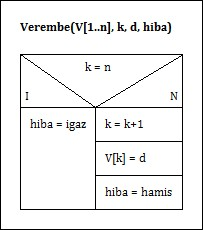
\includegraphics[width=0.3\textwidth]{img/Verembe.jpg}
			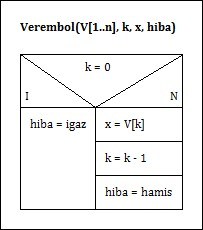
\includegraphics[width=0.3\textwidth]{img/Verembol.jpg}
			\caption{Verem műveletei}
		\end{figure}
		\item \textit{Sor}: Egyszerű, elsőbbségi és kétvégű. A prioritásos sornál az elemekhez tartozik egy érték, ami alapján rendezhetjük  őket.
		\begin{figure}[H]
			\centering
			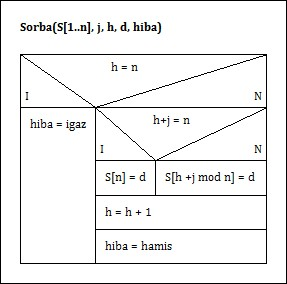
\includegraphics[width=0.3\textwidth]{img/Sorba.jpg}
			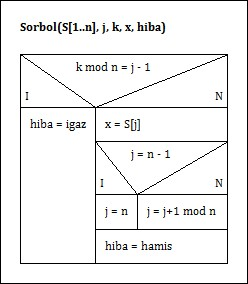
\includegraphics[width=0.3\textwidth]{img/Sorbol.jpg}
			\caption{Sor műveletei}
		\end{figure}
		\item \textit{Lista}: Láncolt ábrázolással reprezentáljuk. 3 szempont szerint különböztethetjük meg a listákat: fejelem van/nincs, láncolás iránya egy/kettő, ciklusosság van/nincs. Ha fejelemes a listánk, akkor a fejelem akkor is létezik, ha üres a lista. \\
		A lista node-okból áll, minden node-nak van egy, a következőre mutató pointere, illetve lehet az előzőre is, ha kétirányú. Ezen kívül van egy első és egy aktuális node-ra mutató pointer is, és az utolsó elem mutatója NIL. A listát megvalósíthatjuk úgy, hogy tetszőleges helyre lehessen elemet beszúrni, illetve törölni.
		\begin{figure}[H]
			\centering
			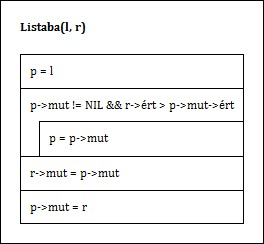
\includegraphics[width=0.3\textwidth]{img/Listaba.jpg}
			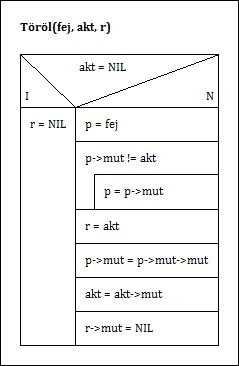
\includegraphics[width=0.3\textwidth]{img/Torol.jpg}
			\caption{Lista műveletei}
		\end{figure}
		\item \textit{Fa}: Egyszerű, bináris és speciális (kupac, bináris keresőfa, AVL-fa). A bináris fát rekurzívan definiáljuk: $t \in T(E)$ [bin. fák típusérték halmaza(alaptípus)] $\iff$ $t$ üres fa (jele: $\Omega$), vagy $t$-nek van gyökéreleme, $bal(t)$, $jobb(t)$ részfája. Láncoltan ábrázoljuk, tömbösen csak teljes fák, illetve kupac esetén.
		\item \textit{Kupac}: Olyan bináris fa, melynek alakja majdnem teljes és balra rendezett. Tömbösen ábrázoljuk, mert pointeresen a bonyolult lépkedést nem teszi lehetővé, tömbösen indexösszefüggésekkel könnyen megoldható.
		\begin{figure}[H]
			\centering
			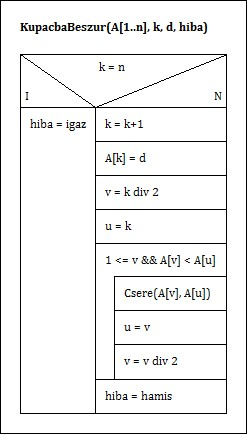
\includegraphics[width=0.3\textwidth]{img/KupacbaBeszur.jpg}
			\caption{Kupac műveletei}
		\end{figure}
		\item \textit{Hasítótábla}
		\item \textit{Gráf} [Nem egyszerű adattípus.]
	\end{itemize}
	
	\subsection{Ábrázolásai}
	
	Absztrakciós szintek:
	\begin{enumerate}
		\item \textit{absztrakt adattípus (ADT)}: specifikáció szintje, itt nincs szerkezeti összefüggés, csak matematikai fogalmak, műveletek logikai axiómákkal vagy előfeltételekkel.
		\begin{itemize}
			\item algebrai (axiomatikus) specifikáció, példa: $Verembe : V \times E \to V$. Axióma, példa: $Felso(Verembe(v,e)) = e$
			\item funkcionális (elő- és utófeltételes) specifikáció, példa: (elsőbbségi) sor $S(E), s \in S$ egy konkrét sor, $s = \{(e_1, t_1), ..., (e_n, t_n)\}$, $n \geq 0$. Ha $n=0$, akkor a sor üres. \\
			$\forall i,j \in [1..n]: i \neq j \to t_i \neq t_j$. \\
			$Sorbol: S \to S \times E$, $\mathcal{D}_{Sorbol} = S \backslash \{ures\}$. Előfeltétel: $Q = (s = s' \wedge s' \neq \emptyset)$, utófeltétel: $R = (s = s' \backslash \{(e,t)\} \wedge (e,t) \in s' \wedge \forall i (e_i, t_i) \in s' : t \leq t_i)$.
		\end{itemize}
		\item \textit{absztrakt adatszerkezet (ADS)}: kognitív pszichológia szintje, ábrák. Az alapvető szerkezeti tulajdonságokat tartalmazza (nem mindet). Ennek a szintnek is része a műveletek halmaza. Példák: az ábra egy irányított gráf, művelet magyarázata, adatszerkezet definiálása.
		\begin{figure}[H]
			\centering
			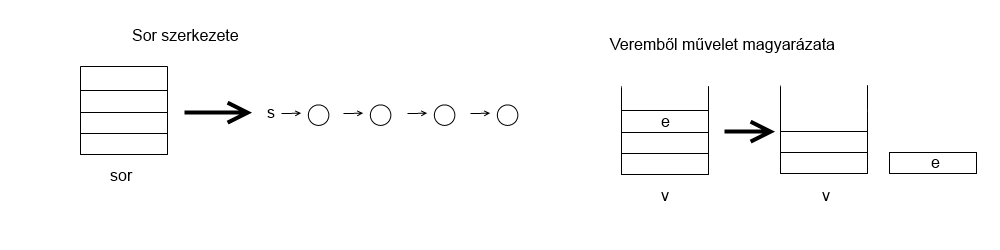
\includegraphics[width=1\textwidth]{img/ads.png}
			\caption{ADS}
		\end{figure}
		\item \textit{ábrázolás/reprezentáció}: döntések (tömbös vagy pointeres ábrázolás), a nyitva hagyott szerkezeti kérdések. Egy adatszerkezetet többféle reprezentációval is meg lehet valósítani (pl. prioritásos sor lehet rendezetlen tömb, rendezett tömb, kupac).
		\begin{itemize}
			\item \textit{tömbös ábrázolás}: takarékos ábrázolás, elhelyezése, tetszőleges rákövetkezések, bejárások, de ezeket meg kell adni.
			\item \textit{pointeres ábrázolás}: minden pointer egy összetett rekord elejére mutat.
		\end{itemize}
		\item \textit{implementálás}
		\item \textit{fizikai szint}
	\end{enumerate}
	
	\subsection{Műveletei}
	
	\begin{itemize}
		\item Üres adatszerkezet létrehozása
		\item Annak lekérdezése, hogy üres-e az adatszerkezet
		\item Elem berakása, itt ellenőrizni kell, hogy nem telt-e még meg
		\item Elem kivétele vagy törlése, itt ellenőrizni kell, hogy nem üres-e
		\item Adott tulajdonságú elem (például maximum, veremben a felső) lekérdezése, itt is ellenőrizni kell, hogy üres-e az adatszerkezet
		\item Bejárások (preorder, inorder, postorder, szintfolytonos), listáknál az első, előző vagy következő elemre lépés
		\item Elem módosítása bizonyos adatszerkezeteknél (pl. listák)
	\end{itemize}
	
	\subsection{Fontosabb alkalmazásai}
	
	\textit{Prioritásos sor}: nagygépes programfuttatásnál az erőforrásokat a prioritás arányában osszuk el, adott pillanatban a maximális prioritásút válasszuk. Sürgősségi ügyeleten, gráfalgoritmusoknál is alkalmazható.
	\textit{B-fa}: ipari méretekben adatbázisokban használják.
	
	\section{A hatékony adattárolás és visszakeresés néhány megvalósítása (bináris keresőfa, AVL-fa, 2-3-fa és B-fa, hasítás (,,hash-elés”))}
	
	\subsection{Bináris keresőfa}
	
	Nincsenek benne azonos kulcsok, a követendő elv: ,,kisebb balra, nagyobb jobbra". Inorder bejárással növekvő kulcssorozatot kapunk. \\
	Műveletigénye fa magasságú nagyságrendű. \\
	Az a cél, hogy a bináris keresőfa ne nyúljon meg láncszerűen, erre jó az AVL-fa és a 2-3-fa.
	\begin{figure}[H]
		\centering
		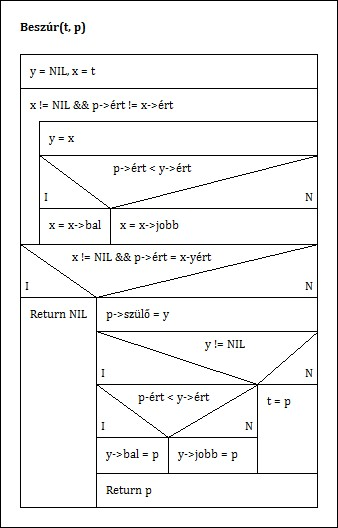
\includegraphics[width=0.3\textwidth]{img/Beszur.jpg}
		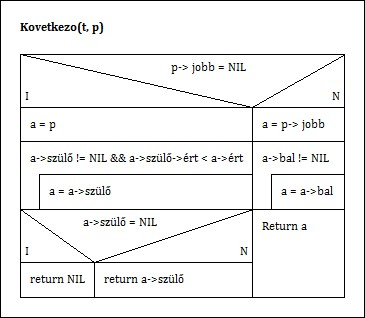
\includegraphics[width=0.3\textwidth]{img/Kovetkezo.jpg}
		\caption{Bináris keresőfa műveletei}
	\end{figure}
	
	\subsection{AVL-fa}
	
	Cél: a $t$ bináris keresőfa magasságának $\log_2(n)$ közelében tartása, azaz $h(t) \leq c \cdot \log_2(n)$, ahol $c$ elfogadhatóan kicsi. Az ilyen fát kiegyensúlyozottnak nevezzük. \\
	\textit{AVL}: Adelszon-Velszkij, Landisz 1962-ben alkották meg. \\
	A $t$ bináris keresőfát egyúttal AVL-fának nevezzük $\iff$ $t$ minden $x$ csúcsára $|h(bal(x))-h(jobb(x))| \leq 1$. \\
	Minden csúcsnak van egy címkéje $+,-,=$ (gyerekek magasságának különbsége). A beszúrás helyétől felfelé ellenőrizzük ezeket, és ha kell, akkor módosítjuk. Ha valahol $++$ vagy $--$ alakul ki, akkor ott elromlik az AVL-tulajdonság, egy vagy több forgatással vagy átkötéssel konstans műveletigénnyel helyre lehet hozni. \\
	Többféle séma is van: $(++,+), (++,-), (++,=)$ és a tükörképeik.
	
	\subsection{2-3-fa és B-fa}
	
	2-3-fa kis méretben az elmélet számára jó, a B-fa a gyakorlati változat adatbázisban. \\
	$t$ 2-3-fa $\iff$ minden belső csúcsnak 2 vagy 3 gyereke van, a levelek azonos szinten helyezkednek el, adatrekordok csak a levelekben vannak, belső pontokban kulcsok és mutatók, levelekben a kulcsok balról jobbra nőnek. \\
	Ha 4 gyerek lenne a beszúrás után, akkor csúcsot kell vágni. Ha törlésnél 1 gyerek lenne valahol, akkor csúcsösszevonásokat és gyerekátadást alkalmazunk. \\
	B-fa nagyobb méretű, itt két határ között mozog a gyerekszám: $\lceil\frac{r}{2}\rceil$ és $r$, ahol $50 \leq r \leq 1000$.
	
	\subsection{Hasítás}
	
	Kulcsos rekordokat tárol.
	\begin{itemize}
		\item \textit{Hasítás láncolással}: a kulcsütközést láncolással oldja fel. Van egy hasítófüggvény: $h: U \to [0..m-1]$, elvárás vele kapcsolatban, hogy gyorsan számolható és egyenletes legyen. $m$-et úgy választjuk meg $n$ nagyságrendjének ismeretében, hogy $\alpha = \frac{n}{m}$ lesz a várható listahossz, ha egyenletes hasítást feltételezünk.\\
		Például kétirányú listát használhatunk a hasításhoz. Műveletek: beszúrás, keresés, törlés. \\
		Gyakorlatban érdemes $m$-et úgy megválasztani, hogy olyan prímszám legyen, ami nem esik 2-hatvány közelébe.
		\item \textit{Hasítás nyitott/nyílt címzéssel}: A kulcsokat lehessen egészként értelmezni, ekkor vannak jó hasítófüggvények. \\
		Próbálkozás általános képlete: $h(k) + h_i(k)$ $(mod$ $M)$, $0 \leq i \leq M-1$. Egész addig alkalmazza, amíg üres helyet nem talál.
		\begin{enumerate}
			\item \textit{Lineáris próba}: $h_i(k) = -i$ $(mod$ $M)$, egyesével balra lépegetve keressük az üres helyet. Hátránya az elsődleges csomósodás, ez jelentős lassulást okoz beszúrásnál és keresésnél.
			\item \textit{Négyzetes próba}: $h_i(k) = (-1)^i(\lceil\frac{i}{2}\rceil)^2$ $(mod$ $M)$, a négyzetszámokkal lépegetünk balra-jobbra, ezek az eltolások kiadják $\{0,1,...,M-1\}$-et. Hátrány: másodlagos csomósodás.
			\item \textit{Kettős hash-elés}: $h_i(k) =-ih'(k)$ $(mod$ $M)$, $h'(k)$ a $k$-hoz tartozó egyedi lépésköz, $(h'(k),M)=1$ relatív prímek. Ha az $M$ elég nagy, akkor nincs csomósodás.
		\end{enumerate}
		\item \textit{Hasítófüggvények}: Leggyakoribb: $k$ egész, kongruencia reláció. Általánosan: $h(k) = (ak +b$ $(mod$ $p))$ $(mod$ $M)$, az univerzális hasítás családja. Tapasztalat: $k$ egyenletesen hasít.
	\end{itemize}
	
	\section{Összehasonlító rendező algoritmusok (buborék és beszúró rendezés, ill. verseny, kupac, gyors és összefésülő rendezés)}
	
	Buborék- és beszúró rendezés klasszikusak, $n^2$-es műveletigényűek, a többi hatékony, $n\log(n)$-es idejűek.
	
	\subsection{Buborékrendezés}
	
	A legnagyobb értéket cserékkel a végéig felbuborékozza, ezt minden ciklus végén elhagyjuk. A gyakorlatban nem használják.
	\begin{figure}[H]
		\centering
		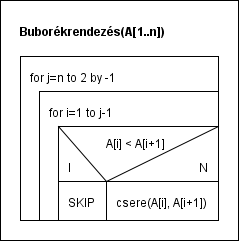
\includegraphics[width=0.3\textwidth]{img/Buborekrendezes.png}
		\caption{Buborékrendezés}
	\end{figure}
	
	\subsection{Beszúró rendezés}
	
	Kis $n$-re (kb 30) ez a rendezés a legjobb. \\
	Itt az elemmozgatás mindig 1 értékadás (buborékrendezésnél a csere 3 értékadás). Listára is implementálni lehet, ez esetben a pointereket állítjuk át, az elemek helyben maradnak. \\
	$A[1..j]$ rendezett, $j=1..n$.
	\begin{figure}[H]
		\centering
		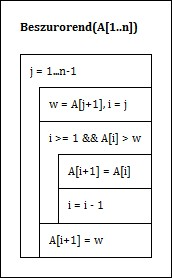
\includegraphics[width=0.3\textwidth]{img/Beszurorend.jpg}
		\caption{Beszúró rendezés}
	\end{figure}
	
	\subsection{Versenyrendezés}
	
	Gyakorlatban nem használják. \\
	Teljes bináris fa az alapja, egy versenyfa. Szintfolytonosan ábrázoljuk tömbösen.\\
	\begin{enumerate}
		\item A versenyfa kitöltése (a verseny lejátszása). Maximum a gyökérben, ennek kiírása az outputra.
		\item $(n-1)$-szer
		\begin{itemize}
			\item[a)] gyökérben szereplő maximális elem helyének megkeresése a levélszinten és $-\infty$ írása a helyére
			\item[b)] az egészet újrajátsszuk (azt az ágat, ahol volt) $\to$ 2. legjobb feljut a gyökérbe
		\end{itemize}
	\end{enumerate}
	\begin{figure}[H]
		\centering
		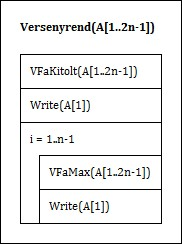
\includegraphics[width=0.3\textwidth]{img/Versenyrend.jpg}
		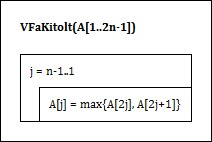
\includegraphics[width=0.3\textwidth]{img/VFaKitolt.jpg}
		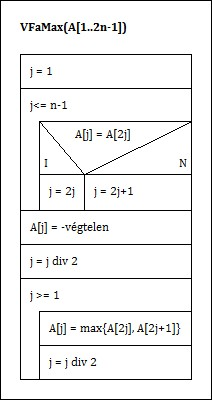
\includegraphics[width=0.3\textwidth]{img/VFaMax.jpg}
		\caption{Versenyrendezés}
	\end{figure}
	
	\subsection{Kupacrendezés}
	
	\begin{enumerate}
		\item Kezdő kupac kialakítása. Rendezetlen input tömbből tartalmi invariánst készítünk, ami már kupac struktúrájú. Elv: cserékkel lesüllyesztjük az elemet a nagyobb gyerek irányába, ha kisebb a nagyobbik gyereknél. A süllyesztés eljuthat ahhoz a csúcshoz, amelynek nincs jobb gyereke.
		\item $(n-1)$-szer
		\begin{itemize}
			\item[a)] gyökérelem és az alsó szint jobb szélső (=utolsó) aktív elemének cseréje, és a csere után lekerült elem inaktívvá tétele
			\item[b)] a gyökérbe került elem süllyesztése az aktív kupacon
		\end{itemize}
	\end{enumerate}	
	\begin{figure}[H]
		\centering
		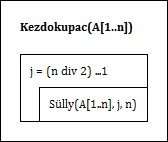
\includegraphics[width=0.3\textwidth]{img/Kezdokupac.jpg}
		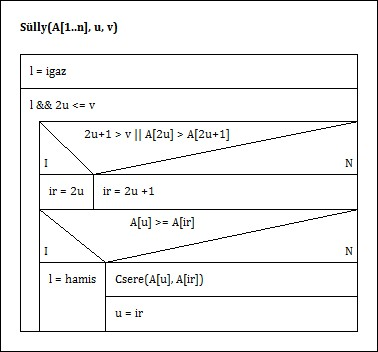
\includegraphics[width=0.3\textwidth]{img/Sully.jpg}
		\includegraphics[width=0.3\textwidth]{img/KupacRend.jpg}
		\caption{Kupacrendezés}
	\end{figure}
	
	A kezdőkupac kialakításánál, és a ciklus közben a süllyesztés módja kicsit különbözik, hiszen az első esetben a változó elem süllyed le a teljes kupacon, a másodikban a gyökér süllyed az aktív kupacon. A képen látható algoritmus mindkét műveletet teljesíti.
	
	\subsection{Gyorsrendezés}
	
	Elve: véletlenül választunk egy elemet. A nála kisebb elemeket tőle balra, a nagyobbakat jobbra rakjuk, az elemet berakjuk a két rész közé. Rekurzív algoritmus.
	\begin{figure}[H]
		\centering
		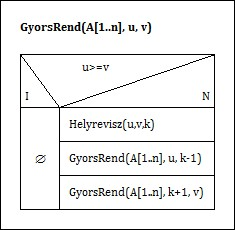
\includegraphics[width=0.3\textwidth]{img/GyorsRend.jpg}
		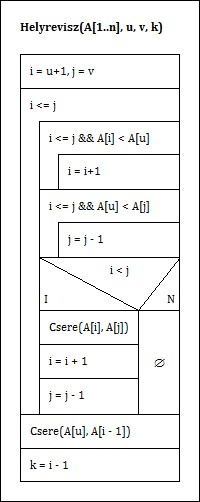
\includegraphics[width=0.3\textwidth]{img/Helyrevisz.jpg}
		\caption{Gyorsrendezés}
	\end{figure}
	
	\subsection{Összefésülő rendezés}
	
	Alapja: 2 rendezett sorozat összefésülése. Ezt alkalmazhatjuk felülről lefelé (rekurzív) vagy alulról felfelé (iteratív), ez utóbbit szekvenciális fájloknál.
	\begin{figure}[H]
		\centering
		\includegraphics[width=0.3\textwidth]{img/OFRend.jpg}
		\caption{Összefésülő rendezés}
	\end{figure}
	
	\section{A műveletigény alsó korlátja összehasonlító rendezésekre}
	
	\subsection{Műveletigény}
	
	Kijelöljük a domináns műveleteket, és az $n$ inputméret függvényében hányszor hajtódnak végre, ezt nézzük. Jelölés általánosan $T(n)$, de lehet konkrétan is, pl $Cs(n)$ [csere]. $mT(n)$ a minimális műveletigény, $MT(n)$ a maximális és $AT(n)$ az átlagos.	
	\begin{itemize}
		\item[$\Theta$]: nagyságrendileg azonos, két konstans közé beszorítható
		\item[$\mathcal{O}$]: nagyságrendi felső becslés, $o$: nincs megengedve az egyenlőség
		\item[$\Omega$]: nagyságrendi alsó becslés, $\omega$: nincs megengedve az egyenlőség
	\end{itemize}
	
	\subsection{Alsókorlát}
	
	Például: $n$ elem maximumkiválasztása legalább $(n-1)$ összehasonlítást igényel. Bizonyítása: Ha ennél kevesebb összehasonlítás lenne, akkor legalább 1 elem kimaradt, és ezzel ellentmondásba kerülhetünk. \\
	\textit{Döntési fa}: Algoritmus $n$ méretű inputra. Kiegyenesednek a ciklusok véges hosszú lánccá, a végrehajtás nyoma egy fa struktúrát ad. Tökéletes fa: minden belső pontnak 2 gyereke van. Ennél az algoritmusnál nincs jobb, mert $2^{h(t)} \geq n!$, összehasonlító rendezés esetén, $n!$ input.
	
	\subsection{Alsókorlát legrosszabb esetben}
	
	Tétel: $MO_R(n) = \Omega(n\log{n})$ A legkedvezőtlenebb permutációra legalább $n\log{n}$ összehasonlítás. Bizonyítás: $\log_2{n!} \leq n\log_2{n} = \Omega(n\log{n})$, és $MO_R(n)=h(t) \geq \log_2{n!}$ (lemma miatt) $\Rightarrow$ $MO_R(n)=\Omega(n\log{n})$.
	
	\subsection{Alsókorlát átlagos esetben}
	
	Legyen minden input egyformán valószínű ($\frac{1}{n!}$). \\
	$AO_R(n) = \frac{1}{n!}\sum_{p \in Perm(n)}{O_R(p)}$, és könnyű belátni, hogy $\sum_{p}{O_R(p)} = lhsum(h(t_R(n)))$ [levél-magasság-összeg]. \\
	Lemma: Az $n!$ levelet tartalmazó tökéletes fák közül azokra a legkisebb az $lhsum(h(t_R(n)))$ érték, amelyek majdnem teljesek. \\
	Tétel: $AO_R(n) = \Omega(n\log{n})$.
	
\end{document}